\documentclass[11pt,reqno]{amsart}
\usepackage[top=1in, left=1in, right=1in, bottom=1in]{geometry}                % See geometry.pdf to learn the layout options. There are lots.
\geometry{letterpaper}                   % ... or a4paper or a5paper or ...
\usepackage[parfill]{parskip}    % Activate to begin paragraphs with an empty line rather than an indent

\usepackage{algorithm}
\usepackage{algpseudocode}
\usepackage{hyperref}
\usepackage{graphicx}
\usepackage{url}
\usepackage{verbatim}
\usepackage{amssymb}
\usepackage{amsaddr}
\usepackage{amsmath}
\usepackage{enumitem}
\usepackage{setspace}
\usepackage{natbib}
\usepackage{booktabs}
\usepackage{lscape}
\usepackage{threeparttable}

\newcommand{\RR}{I\!\!R} %real numbers
\DeclareMathOperator{\diag}{diag}

\algnewcommand{\Inputs}[1]{%
  \State \textbf{Inputs:}
  \Statex \hspace*{\algorithmicindent}\parbox[t]{.8\linewidth}{\raggedright #1}
}
\algnewcommand{\Initialize}[1]{%
  \State \textbf{Initialize:}
  \Statex \hspace*{\algorithmicindent}\parbox[t]{.8\linewidth}{\raggedright #1}
}


%\title[Reveiw on RVD Methods]{Review on rare genetic variant detection methods for next-generation sequencing data}
\title[Review on RVD Methods in cfDNA NGS]{Review on Rare Variant Detection Methods for Cell-free DNA in Next-generation Sequencing Data}
\author[F. Zhang AND P. Flaherty]{Fan Zhang\,$^{1}$, Patrick Flaherty\,$^{1,2}$}
\address{$^{1}$Department of Biomedical Engineering, Worcester Polytechnic Institute, MA, USA\\
$^{2}$Department of Mathematics and Statistics, University of Massachusetts, Amherst, MA, USA}

\begin{document}
\maketitle

\section{Introduction}
%\subsection{Sequence Analysis Pipeline}
%Scope of the article: nucleotides and variant calling in the context of larger pipeline.
Next-generation sequencing (NGS) technology has revealed the presence of extensive genomic variants in clinical samples.
In general, genomic variants can be present in the form of single nucleotide variants (SNVs), insertions and deletions, structural variants, and copy number variations.
Single nucleotide variant is a primary source of genetic variation that can cause susceptibility to disease or drug resistance to  anti-tumour therapeutics.
The general pipeline to analyze single nucleotide variants in the large-scale NGS data basically consists five main steps: quality control, preprocessing, alignment, post-alignment processing, and variant analysis ~\citep{Bao2014}.
Variant analysis basically contains three main parts: variant detection, annotation, and visualization, among which variant detection is crucial for NGS data analysis with an objective of discovering disease-causing variants.


%Detection in cell free DNA using NGS 
Cell-free DNA (cfDNA) next-generation sequencing has been performed to accurately detect genetic variants that can be used as biomarkers for early cancer detection and anti-cancer treatment monitoring ~\citep{schwarzenbach2011cell, zhou2014pilot}.
It has been demonstrated that cfDNA sequencing is able to detect tumor-derived variants with high sensitivity and specificity in the frequently mutated genes in pancreatobiliary tumor samples ~\citep{zill2015cell}.
However, it is an challenge to detect the variants in cfDNA due to the low allele frequencies occured in tumor samples.
Another reason is the low fraction of cfDNA and the dilution effect of the normal DNA in the blood. 
Thus, bioinformatics methods for cfDNA sequencing analysis are more than desirable to analyze and interpret the rare variants that are relevant to cancer diagnostic and prognostic.


%Outline the paper here with one paragraph overview per section.
In this review, we focus on single nucleotide variant detection in cfDNA next-generation sequencing data and classification of current computational and statistical variant detection methods.
We first highlight the necessity of a sensitive variant detection method from the perspective of biological impacts and statistical accuracy,
and then present the hallmarks of a good variant detection method based on the evaluation of accuracy, scalability, and robustness.
We also discuss the issues that will effect the ability of variant detection methods.
Finally, we classify the state-of-the-art variant detection methods into the categories of probabilistic and non-probabilistic methods and survey each method in detail.


\section{Variant detection in cell-free DNA sequencing data}

NGS of cfDNA is a non-invasive method for tumor-associated or drug resistant variants detection, which will be highly promising for detecting clinical biomarkers and monitoring therapy responses. 
Many remarkable variants on tumor-specific genes, such as \textit{TP53}, \textit{BRAF}, and \textit{KRAS}, can be observed on cfDNA.
\citet{shinozaki2007utility} first detected \textit{BRAF} variant V600E on cfDNA at different stages and demonstrated its clinical use for monitoring behavior of melanoma patients.
Theses clinically relevent variants can be taken as candidate biomarkers and identification of these variants are required to monitor the response to treatment.

We summarize the workflow of variant detection in cfDNA NGS data in Figure \ref{fig:flowchart}.
CfDNA is first extracted from plasma where tumor cfDNA (blue curves) and normal cfDNA (green curves) are mixed together.
After library construction and sequencing process, reads are aligned to the reference genome to prepare for alteration detection.
Then, a rare variant detection method is needed to identify the single nucleotide variants in the dfDNA sequencing data.
Finally, tumor-associated variants are obtained and can be further interpreted for clinical utility.


\begin{figure}[htbp]
\centering
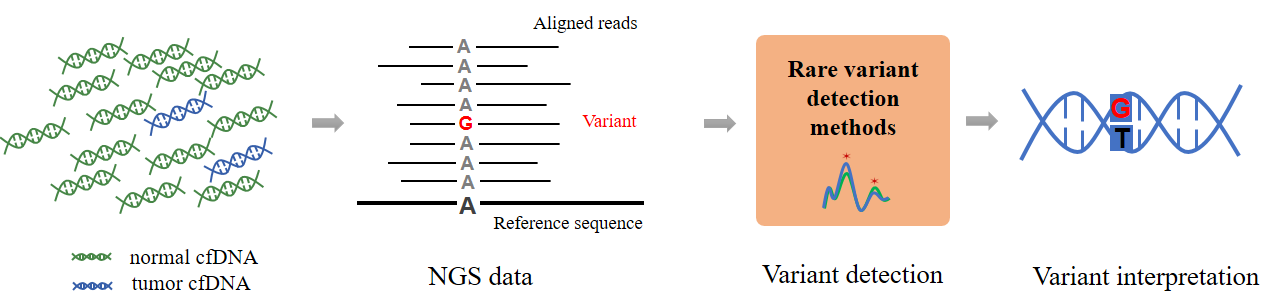
\includegraphics[width=1\textwidth]{flowchart.png}
\caption{Flowchart of variant detection on cfDNA from NGS data.}
\label{fig:flowchart}
\end{figure}



\section{Why do we need a sensitive variant detection method?}

\subsection{Biological impacts}

The cost of whole-genome sequence (WGS) or whole-exome sequence (WES) has been reduced to below $\$1000$, which has made it possible to have a deeper understanding of the structure of genomes to improve the effectiveness of disease treatment. 
The bottleneck of large-scale sequencing is accurate and efficient data analysis rather than data generation.
Most variants revealed by the WGS and WES are demonstrated to be rare by 1000 Genomes ~\citep{10002010map} and rare variants do cause risk of disease or have large effects ~\citep{kosmicki2016discovery}.
The oseltamivir resistance variant, H275Y, exists in a fraction of $0.18\%$ in a clinical sample ~\citep{Flaherty2012}.
A accurate and sensitive variant detection method is needed to identify this causal variant to improve the efficacy of antiviral therapy.
Detection of variants in low fraction of cfDNA will be effective and efficient in monitoring tumor progression, which will be a complement to the cancer tissue biopsies.
A pilot study has shown the feasibility of leukemic cfDNA to be used to resolve DNA abnormalities ~\citep{zhou2014pilot}.
Therefore, a sensitive computational method is a critical step to accelerate rare variants detection and interpretation in the cfDNA data in order to derive further biological inference.


\subsection{Statistical accuracy}

Since the allele frequency of rare variants in the public genomes data is relatively low, it needs methods with high statistical power to identify rare variants in impure samples. 
It is also difficult to guarante statistical accuracy for low or moderate sequencing read depths because simple strategies based on cutoffs for counting alleles may lead to wrong prediction.
To achieve high statistical accuracy, statistical and probabilistic methods have been appeared and mature in providing measures of uncertainty for genotypes inference in variant detection ~\citep{Nielsen2011}.  
Specifically, Bayesian statistical methods are popular for developing sensitive variant detection tools by incorporating proper prior probabilities of possible genotypes and afterwards predict the true genotype using a maximum a posteriori probability (MAP).
Several studies have used a binomial probabilistic distribution to model the sequencing error distribution that can be further used to differentiate errors from the true biological variants ~\citep{Flaherty2012, Shiraishi2013, gerstung2012reliable, Christoforides2013}.



\section{Hallmarks of a good variant detection method}

\subsection{Accuracy}

Accuracy is normally taken as the first criteria to evaluate the performance of a variant detection method.

choose proper prior 

\subsection{Scalability}

Much efforts have been devoted to improve the scalability since analyzing the NGS sequencing data, especially those WGS and WES data, is truly time consuming.
Performing statistical inference and estimation for statistical variant detection methods, such as Bayesian and heuristic, is a process of drawing conclusions of variant detection from the data. 
MCMC sampling algorithm is comprehensively used for statistical inference, but the limitation of MCMC is that the time to converge can be long and the convergence can be hard to diagnose.
Alternatively, variational approxiamtion algorithm converges faster than the MCMC sampling algorithm because it yields deterministic approximation that provides buonds on probability of interest instead of stochastic sampling ~\citep{jordan1999introduction}.
For example, mean field algorithm is a variational approximation method which is demonstrated to be 10 to 30 times faster than the MCMC sampling while producing the same accuracy ~\citep{peterson1989explorations}.
\citet{flaherty2005latent} has used a variational algorithm to estimate the model for chemogenomic profiling.
However, from the perspective of parallel programming, sampling-based methods are easy to be ditributed to multiple computing cores in parallel even though the algorithm itself is computationally slow.
There has to be a tradeoff between accuracy and scalability and accuracy generally takes priority over scalaility.
Balance of accuracy and scalability often depends on specific purposes and resources.

\subsection{Robustness}

The ability to handle noise, contaminate data

Robust Bayesian analysis about sensitivity of Bayesian to study the uncertainty of prior distributions.



\section{Factors that affect the ability of variant detection methods}
The next-generation sequencing data is massive and heterogeneous and many factors could influence the performance of a variant detection method.
\subsection{Quality control}
The quality of the data can affect variant detection, so checking the quality of the raw data and filtering the low-confidence alleles in advance will improve the accuracy of variant detection.
A standard tool, FastQC, is implemented for assessing the quality by generating analytical graphs.
Low-confidence alleles can be trimmed using a standalone tool, NGS QC Toolkit ~\citep{patel2012ngs}, to prevent from making a wrong variant call.
Although filtering low-confidence alleles helps with read alignment, it is noticeable that false positives could be introduced for high-coverage data set ~\citep{liu2012steps}.
Thus, we should consider not only quality control in read mapping but also the read depth of coverage in order to ensure the accuracy of variant detection.

\subsection{Depth of coverage}
Sequencing depth of coverage, number of times that each base has been sequenced, contributes to the results of variant detection because sufficient depth of coverage is necessary to support an accurate variant call.
Due to the high cost of sequencing, the depth of coverage of the sequencing data can be low (less than $10\times$) and the distribution of the read depth over each site could be not uniform.
Previous researchers have studied the effect of coverage and revealed that high coverage data leads to high sensitivity of variant detection ~\citep{neuman2013analysis, krawitz2010microindel}.
~\citep{liu2013variant} indicates that the false discovery rate of variant detection using GATK decreased as the depth of coverage increased.
Generally, the minimum coverage for a single nucleotide polymorphism is 50x and some applications may need higher coverage ~\citep{Schlotterer2014}.
It is reasonable that if you desire to detect a rare variant of $0.1 \%$ allele frequency, the required depth of coverage $1000\times$.
Furthermore, unmatched sequencing read depths of case and control samples will result in increased false positives ~\citep{garner2011confounded}.
%Develop probabilistic methods to estimate the posterior probability of each site to be a variant in the low read depth data.

\subsection{Sequencing errors}
Intrinsic errors from next-generation sequencing platform exist in sample processing and sequencing ~\citep{Olson2015}.
These errors may cause false positives and false negatives in the variant detection step.
Especially, identification of variants of minor variant allele frequency (VAF) is challenging because it is difficult to differentiate a true rare variant (VAF $<$1 \%) from a common sequencing error rate (1\% $<$ VAF $<$ 3\%).
% give an example error from sample processing
% give an example error from sequencing
% give an example error from variant detection
In variant detection step, errors may also exist due to the limitation of the design of the variant detection methods.
For example, a prior assignment in a probabilistic method can be subjective, which may cause bias to predict the probabilistic distribution of the allele frequency of a site in the sequence.
This will lead a miscalling of a rare variant when comparing the allele frequencies of one site in a control/case pair.

\subsection{Sample size}
Multiple samples (pooled sequencing) enabled us to identify more rare variants than individual sample ~\citep{Bao2014, liu2012steps}.
~\citep{liu2013variant} demonstrated that GATK gives higher sensitivity for variant detection in a multiple-sample strategy than a single-sample strategy, but the specificity turned out to be decreased in multiple-sample strategy.
The reason is that more false positives are called in larger data sets with multiple samples ~\citep{Nielsen2011}.
However, if the coverage of the multiple samples is low, the false discovery rate for variant detection could be increased compared with the case of high coverage ~\citep{Cheng2014}.
~\citep{le2011snp} observed that large data set of multiple sequencing samples at low coverage (4-6$\times$) yields higher capability in rare variant detection compared to small data set of less sequencing samples at high coverage.

\section{Classification for variant detection methods}
We classify the state-of-the-art variant detection methods into two categories - probabilistic methods, and non-probabilistics or other combination (Table \ref{tbl:methods}).
We discuss every method from three aspects: specific purpose of the method, category that this method falls into, and metrics or its applications.

%\begin{table}[htbp]
%\centering
%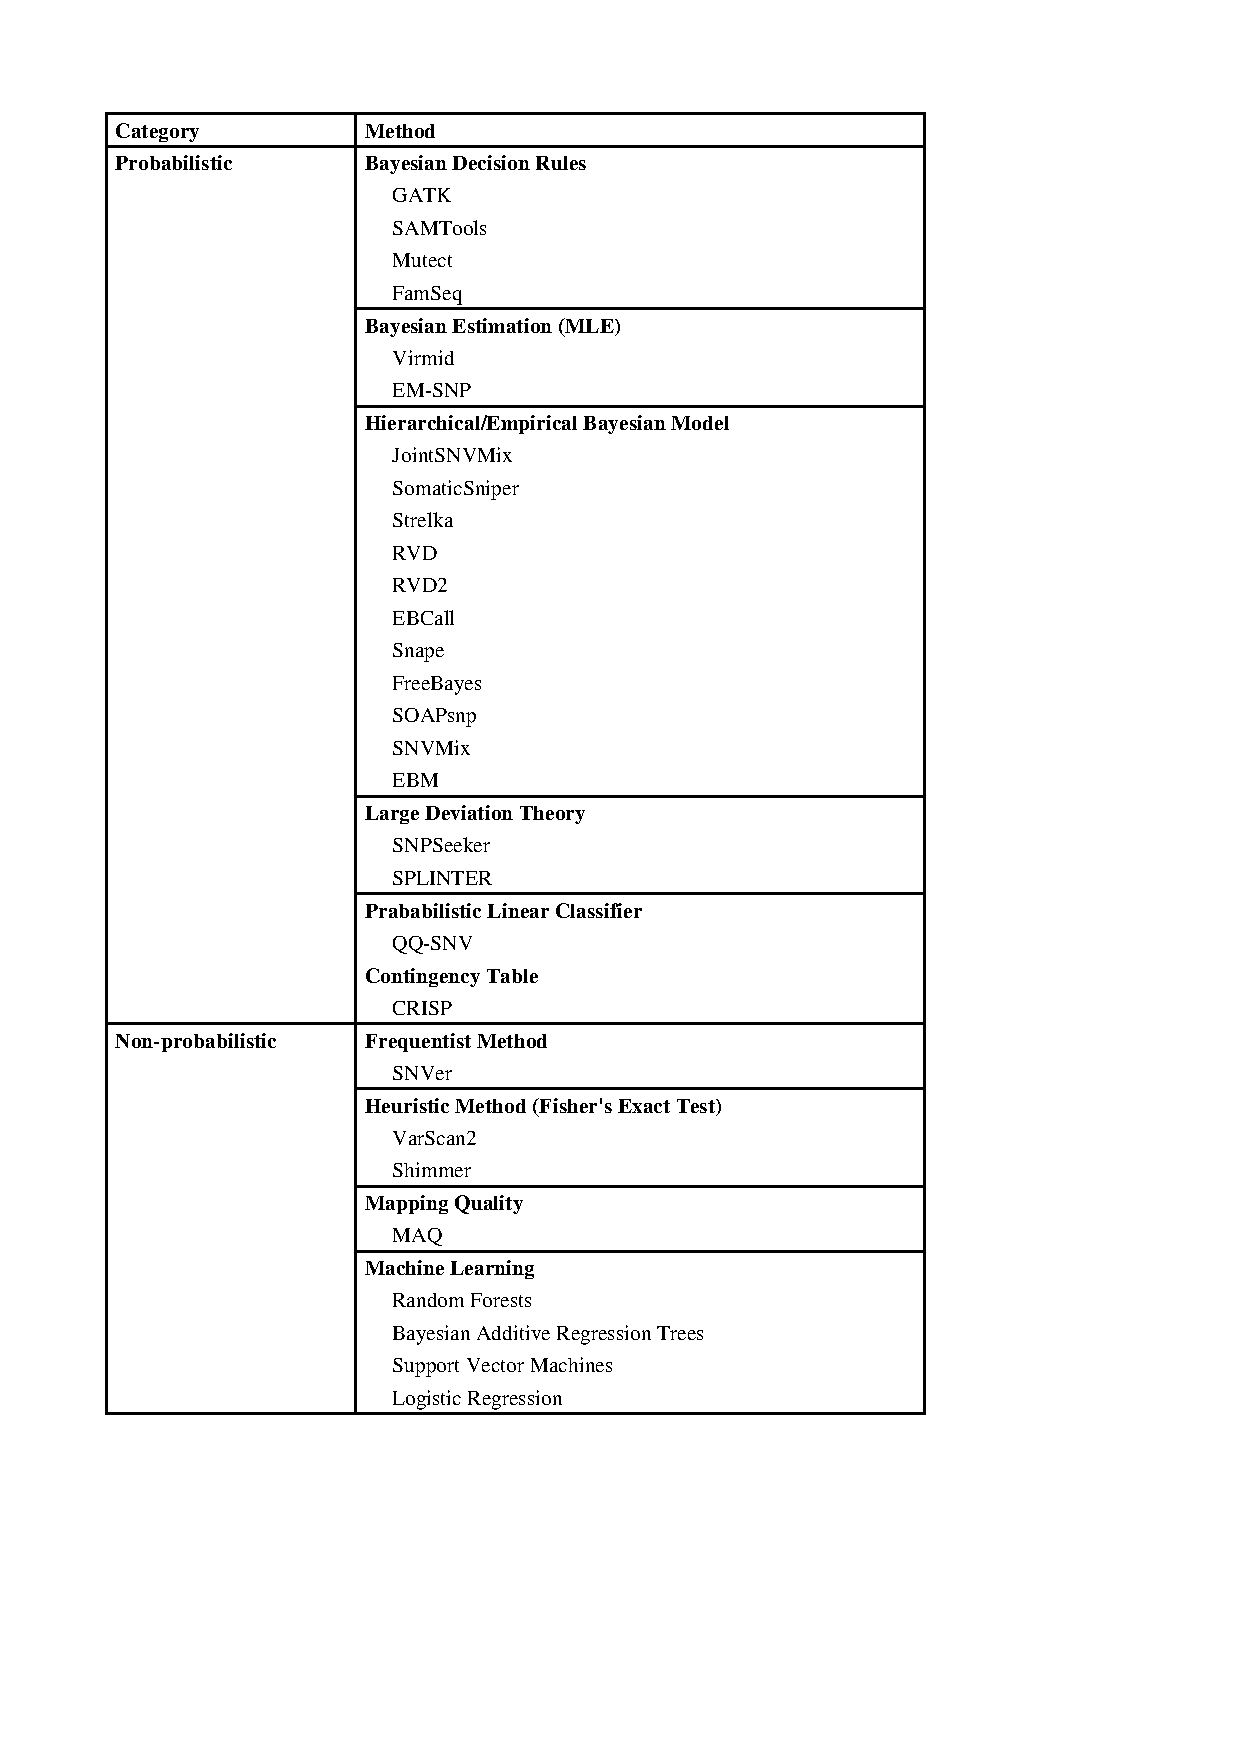
\includegraphics[width=0.9\textwidth]{method_table.pdf}
%\caption{Single nucleotide variant detection methods.}
%\label{tbl:methods}
%\end{table}

%\begin{table}[htbp]
%  \centering
%  \caption{Classification of variant detection methods in next-generation sequencing data.}\label{tbl:methods}
%  \footnotesize
%    \begin{tabular}{rr}
%    \toprule
%    \textbf{Category} & \textbf{Subcategory} & \multicolumn{1}{l}{\textbf{Method}} \\
%    \midrule
%    \textbf{Probabilistic} & \textbf{Bayesian Decision Rules} & \multicolumn{1}{l}{\quad GATK} \\
%          & \multicolumn{1}{l}{\quad SAMTools} \\
%          & \multicolumn{1}{l}{\quad Mutect} \\
%          & \multicolumn{1}{l}{\quad FamSeq} \\
%          & \multicolumn{1}{l}{\textbf{Bayesian Estimation}} \\
%          & \multicolumn{1}{l}{\quad Virmid} \\
%          & \multicolumn{1}{l}{\quad EM-SNP} \\
%          & \multicolumn{1}{l}{\textbf{Hierarchical/Empirical Bayesian}} \\
%          & \multicolumn{1}{l}{\quad JointSNVMix} \\
%          & \multicolumn{1}{l}{\quad SomaticSniper} \\
%          & \multicolumn{1}{l}{\quad Strelka} \\
%          & \multicolumn{1}{l}{\quad RVD/RVD2/Variational RVD} \\
%          & \multicolumn{1}{l}{\quad EBCall} \\
%          & \multicolumn{1}{l}{\quad Snape} \\
%          & \multicolumn{1}{l}{\quad FreeBayes} \\
%          & \multicolumn{1}{l}{\quad Seurat} \\
%          & \multicolumn{1}{l}{\quad DeepSNV} \\
%          & \multicolumn{1}{l}{\quad SOAPsnp} \\
%          & \multicolumn{1}{l}{\quad SNVMix} \\
%          & \multicolumn{1}{l}{\quad EBM} \\
%          & \multicolumn{1}{l}{\textbf{Large Deviation Theory}} \\
%          & \multicolumn{1}{l}{\quad SNPSeeker} \\
%          & \multicolumn{1}{l}{\quad SPLINTER} \\
%          & \multicolumn{1}{l}{\textbf{Prababilistic Linear Classifier }} \\
%          & \multicolumn{1}{l}{\quad QQ-SNV} \\
%          & \multicolumn{1}{l}{\textbf{Contingency Table }} \\
%          & \multicolumn{1}{l}{\quad CRISP} \\
%          \midrule
%    \textbf{Non-probabilistic} & \multicolumn{1}{l}{\textbf{Frequentist Method}} \\
%    \textbf{or other combination} & \multicolumn{1}{l}{\quad SNVer} \\
%         & \multicolumn{1}{l}{\textbf{Heuristic Method}} \\
%         & \multicolumn{1}{l}{\quad VarScan2} \\
%         & \multicolumn{1}{l}{\quad Shimmer} \\
%         %& \multicolumn{1}{l}{\textbf{Mapping Quality}} \\
%         %& \multicolumn{1}{l}{\quad MAQ} \\
%         & \multicolumn{1}{l}{\textbf{Machine Learning}} \\
%         & \multicolumn{1}{l}{\quad Atlas2} \\
%         & \multicolumn{1}{l}{\quad Feature-based methods} \\
%    \bottomrule
%    \end{tabular}
%\end{table}


\begin{landscape}
\begin{table}[htbp]
  \centering
  \tiny
  \caption{A summary of the state-of-the-art variant detection methods for NGS data and the category classification of them.}\label{tbl:methods}
  \begin{threeparttable}
    \begin{tabular}{rllllr}
    \multicolumn{1}{l}{\textbf{ Category}} & \textbf{Subcategory/Method} & \textbf{Functions} & \textbf{Platform} & \textbf{Source Code} & \multicolumn{1}{l}{\textbf{Ref}} \\
    \toprule
    \multicolumn{1}{l}{\textbf{ Probabilistic}} & \textbf{Bayesian Decision Rules} &       &       &       &  \\
          & GATK  & SNVs, indels   & Java  & https://www.broadinstitute.org/gatk/ & \citealt{McKenna2010} \\
          & Mutect & SNVs  & Java  & http://www.broadinstitute.org/cancer/cga/mutect & \citealt{Cibulskis2013} \\
          & SAMTools & SNVs, indels  & C     & http://samtools.sourceforge.net/ & \citealt{Li2009a} \\
          & FamSeq & SNVs  & C++   & http://bioinformatics.mdanderson.org/main/FamSeq &  \citealt{Peng2013}\\
          & MAQ & SNVs & Perl & http://maq.sourceforge.net/ & \citealt{Li2008}\\
          & JointSNVMix & SNVs  & Python & http://compbio.bccrc.ca/software/jointsnvmix/ & \citealt{Roth2012} \\
          & \textbf{Bayesian Estimation} &       &       &       &  \\
          & Virmid & SNVs  & Java  & https://sourceforge.net/projects/virmid/ & \citealt{Kim2013} \\
          & EM-SNP & SNVs  & R     & http://www-rcf.usc.edu/~fsun/Programs/EM-SNP/EM-SNP.html &  \citealt{Chen2013}\\
          & \textbf{Bayesian } &       &       &       &  \\
          & SomaticSniper & SNVs  & Perl  & http://gmt.genome.wustl.edu/packages/somatic-sniper/ &  \citealt{Larson2012}\\
          & Strelka & SNVs, indels & Perl  & https://sites.google.com/site/strelkasomaticvariantcaller/ &  \citealt{Saunders2012}\\
          & RVD/RVD2/VI RVD & SNVs  & Python & http://genomics.wpi.edu/rvd2/ &  \citealt{He2015}\\
          & FreeBayes & SNVs, indels & Python & https://github.com/ekg/freebayes & \citealt{Garrison2012} \\
          & EBCall & SNVs, indels & R     & https://github.com/friend1ws/EBCall &  \citealt{Shiraishi2013}\\
          & DeepSNV & SNVs  & R     & http://www.bioconductor.org/packages/release/bioc/html/deepSNV.html &  \citealt{gerstung2012reliable}\\
          & EBM   & SNVs  & R     & https://sites.google.com/site/zhouby98/ebm & \citealt{Zhou2012} \\
          & Snape & SNVs  & C     & https://code.google.com/archive/p/snape-pooled/ &  \citealt{Raineri2012}\\
          & SNVMix & SNVs  & C     & http://compbio.bccrc.ca/software/snvmix/ & \citealt{Goya2010} \\
          & SOAPsnp & SNVs  & C, C++ & http://soap.genomics.org.cn/soapsnp.html &  \citealt{Li2009}\\
          & Seurat & SNVs  & Java  & https://sites.google.com/site/seuratsomatic/ &  \citealt{Christoforides2013}\\
          & \textbf{Likelihood-based} &       &       &       &  \\      
          & glfTools & SNVs  & C, C++  & csg.sph.umich.edu//abecasis/glfTools/ &  \citealt{abecasis2010}\\    
          & PolyMutt & SNVs, indels  & C++  & http://genome.sph.umich.edu/wiki/Polymutt &  \citealt{li2012likelihood}\\           
          & \textbf{Large Deviation Theory} &       &       &       &  \\
          & SNPSeeker & SNVs  & C     & http://genetics.wustl.edu/rmlab/software/ &  \citealt{Druley2009}\\
          & SPLINTER & SNVs, indels & C, C++ & available on request &  \citealt{Spencer2014}\\
          & \textbf{Linear Classifier } &       &       &       &  \\
          & QQ-SNV & SNVs  & Perl  & https://sourceforge.net/projects/qqsnv/ & \citealt{VanderBorght2015} \\
          & \textbf{Contingency Table } &       &       &       &  \\
          & CRISP & SNVs  & Ptython & https://sites.google.com/site/vibansal/software/crisp & \citealt{Bansal2010}  \\
    \multicolumn{1}{l}{\textbf{Non-probabilistic }} & \textbf{Frequentist Method} &       &       &       &  \\
    \multicolumn{1}{l}{\textbf{or}} & SNVer & SNVs  & Java  & http://snver.sourceforge.net/ &  \citealt{Wei2011}\\
    \multicolumn{1}{l}{\textbf{other cambination}} & \textbf{Heuristic Method } &       &       &       &  \\
          & VarScan2 & SNVs, indels & Java  & http://varscan.sourceforge.net/ & \citealt{Koboldt2012} \\
          & Shimmer & SNVs  & Perl  & https://github.com/nhansen/Shimmer & \citealt{Hansen2013} \\
          & \textbf{Machine Learning } &       &       &       &  \\
          & Atlas2 & SNVs, indels  & Ruby  & https://sourceforge.net/projects/atlas2/ &  \citealt{challis2012integrative}\\
          & Feature-based methods & SNVs  & Python & http://compbio.bccrc.ca/software/mutationseq/ &  \citealt{Ding2012}\\
    \bottomrule
    \end{tabular}
    \begin{tablenotes}
	\item Category and subcategory of each variant detection method is classified into. 
Fuctions for identifying SNVs and indels are distinguished. SNVs, single nucleotide variants; indels, insertions/deletions.
Platforms of languages and source code are given.
    \end{tablenotes}
\end{threeparttable}
\end{table}
\end{landscape}





\subsection{Probabilistic methods}
We summary 22 variant detection methods that are developed based on probabilistic strategy in detail.

\textbf{GATK} ~\citep{McKenna2010} is designed for detecting germline variants in homogeneous samples.
It uses a simple Bayesian genotyper to calculate the posterior distribution of each genotype given mapped reads over each site ~\citep{depristo2011framework}.
It adopted a MapReduce system to facilitate processing large-scale sequencing data in parallel and has been involved in 1000 Genomes Project and The Cancer Genome Atlas.

\textbf{MuTect} ~\citep{Cibulskis2013} is a method to detect germline and somatic variants with low allele frequencies at various sequencing read depths in mixed tumour samples.
It is built on a Bayesian classifier to calculate a log-likelihood ratio that can be used as a threshold for variant detection in matched tumour and normal samples.
It has been shown that MuTect is more sensitive than other competing methods in detecting somatic variants within low fraction of tumour cells, which enables us to discover subclonal drivers for tumour progression.

Mapping and assemblly with quality (\textbf{MAQ}) ~\citep{Li2008} is a probabilistic method that used a fixed prior for estimation of non-reference allele probabilities.
\textbf{SAMtools} ~\citep{Li2009a} is a revised MAQ model to manipulate the genomic sequences in the SAM and BAM format.
Similar to GATK, SAMtools computes the likelihood of each possible genotype using a naive Bayesian model and then identifies germline variants using BCFtools ~\citep{li2011statistical}.
It has been demonstrated for comparable accuracy in real data for allele count estimation, allele frequency estimation, and association mapping.
\textbf{glftools} ~\citep{abecasis2010} is a revised version of SAMtools to generate genotype likelihood files.
Single individual, glfSingle and mltiple individuals, glfMultiples are developed for genotype calling as well.

\textbf{FamSeq} ~\citep{Peng2013} is a family-based sequencing program for variant detection in the data of family members.
FamSeq uses Bayesian network to yield posterior probabilities for measure of genotype calls and MCMC sampling method to derive the posterior probabilities.
This method integrates Mendelian inheritance and sequencing data of family members to reduce the false positive rate and false negative rate for variant detection.

\textbf{JointSNVMix} ~\citep{Roth2012} is introduced to discover somatic point variants and distinguish germline from somatic events.
It applies two novel Bayesian probabilistic models to jointly analyze the allelic count of tumour and normal samples.
Concordance is used as a probabilistic threshold to measure the performance of variant detection.
Is has been demonstrated that the joint modeling, JointSNVMix, has higher specificity than its independent analogue with guaranteed sensitivity.

\textbf{Virmid} ~\citep{Kim2013} is implemented for somatic variant detection using the idea of estimating the level of sample contamination.
Maximum likelihood estimation is used for sample impurity estimation and joint genotype probability estimation, and Bayesian inference is used for variant detection.
The strategy of estimating the level of contamination helps to reduce computational running time and increase accuracy in variant detection.

\textbf{EM-SNP} ~\citep{Chen2013} can be used for allele frequency estimation, SNVs detection and association study in pooled sequencing data.
They developed an expectation maximization (EM) algorithm to approximate the maximum likelihood of the parameters to estimate the minor allele frequencies.
It has been shown that EM-SNP outperforms SNVer in rare variants detection in the type 1 diabetes pooled sequencing data by comparison on the metrics of dbSNP and transition/transversion ratio.


\textbf{SomaticSniper} ~\citep{Larson2012} detects somatic variants by directly comparing the joint diploid genotype likelihoods for a tumour-normal pair.
The genotype likelihood is calculated using MAQ method ~\citep{Li2008} by incorporating the dependency of the genotypes between tumour and normal samples.
Sensitivity and precision are employed to evaluate the performance of variant detection on a simulated data set.

\textbf{Strelka} ~\citep{Saunders2012} is an algorithm for somatic variant detection in a joint analysis of matched tumour and normal samples.
It is a Bayesian method that models the joint probabilistic distribution of continuous allele frequencies.
Strelka is capable to maintain high sensitivity in low purity tumour samples.

\textbf{FreeBayes} ~\citep{Garrison2012} is a haplotype-based variant detection method for short read DNA sequencing data.
It is a generalization of a Bayesian statistical method ~\citep{marth1999general} to detect variants in both individual and pooled samples.
A gradient ascent method is employed to establish a maximum a posteriori (MAP) estimate of the genotype for each sample.
This framework is able to identify longer and multi-alleles by modeling multiallelic site.

\textbf{EBCall} ~\citep{Shiraishi2013} is proposed to detect somatic variants by incorporating sequencing errors as prior information into the model.
It is developed based on an empirical Bayesian framework where Beta-Binomial distribution is used to depict sequencing errors.
EBCall can detect somatic variants of less than 10\% allele frequencies in tumour subclones.

\textbf{DeepSNV} ~\citep{gerstung2012reliable} is a powerful statistical method for detecting SNVs in ultra-deep sequencing data.
This algorithm is built on a hierarchical beta-binomial model and a likelihood ratio test is calculated for each base for comparison with a control or a reference.
DeepSNV is validated on subclonal diverse tumour samples of renal cell carcinoma and reveals an agreement of the variant allele frequencies of the variants with the original work ~\citep{gerstung2012reliable}.

\textbf{EBM} ~\citep{Zhou2012} aims to detect SNVs in pooled sequencing data by accurately estimating the sequencing error distribution across multiple pools and genomic positions. 
It is a empirical Bayes mixture model and an expectation-conditional maximization (ECM) algorithm is used for model inference and parameter estimation.
It is demonstrated with lower sum of squared errors of the estimated allele frequencies compared with a naive estimator.


\textbf{Snape} ~\citep{Raineri2012} is built to detect SNVs in pooled samples.
It is a Bayesian method that takes into account of different priors to estimate the posterior frequency probability of SNVs.
Snape has low false discovery rate and high power on a simulated data set that is generated by ART ~\citep{huang2012art}.

\textbf{SNVMix} ~\citep{Goya2010} is a probabilistic method to detect SNVs from tumour NGS data.
It is developed based on Binomial mixture models and an expectation maximization algorithm is used to obtain model parameters to predict allele frequencies.
It is demonstrated with high sensitivity and specificity on a breast cancer data set of $> 40 \times$ that the ground truth of SNVs is known.

\textbf{SOAPsnp} ~\citep{Li2009} is a variant detection method that is designed for massively parallel sequencing-by-synthesis Illumina Genome Analyzer data.
It uses a Bayesian statistical model to infer the likelihood of each possible genotype and outputs the genotype with highest posterior proabability for each site.
it achieves high accuracy in a human genome deep resequencing data and incorparating dbSNP genotypes as prior information helps with identify real heterozygotes in low read depth data.

\textbf{Seurat} ~\citep{Christoforides2013} aims to detect somatic events, including SNVs, insertion/deletions, and structural variations, within tumors in paired tumor and normal samples.
Seurat is a generalized Bayesian framework that uses a beta-binomial distribution to model the probability of a somatic event.
Seurat shows high transition/transversion ratio, low non-synonymous/synonymous ratio, and low dbSNP rate on a lymphoma tumor data set, which demonstrates that Seurat has high specificity.

\textbf{PolyMutt} ~\citep{li2012likelihood} is a likelihood based method to detect novel SNVs in samples of families.
PolyMutt models likelihood of reads in pedigrees using the Elston-Stewart algorithm ~\citep{elston1971general}.
It has been shown that the information from families help to improve the specificity for SNVs detection in a simulations study.

\textbf{SNPSeeker} ~\citep{Druley2009} used the large deviation theory to detect SNVs from large pool of multiple individuals.
Negative control data is necessary for model estimation.
It is able to detect the SNVs that present with lower allele frequencies than the error rate of the sequencing platform.

\textbf{SPLINTER} ~\citep{Spencer2014} is based on the large deviation theory to detect rare alleles in pooled sequencing samples.
This research shows that over $500 \times$ coverage is a guarantee for an ideal performance to detect low frequency variants ($25\% - 2.5\%$) on a synthetic DNA mixture of HapMap samples.
It also reveals that SPLINTER has acceptable specificity and positive predictive value (PPV) in clinical sequencing regions.

\textbf{QQ-SNV} ~\citep{VanderBorght2015} is developed to differentiate true SNVs from errors using the quantiles of the quality scores.
Instead of modeling the position-specific allele frequency, a logistic regression classifier model is used to classify a position as a variant or an error by incorporating the Illumina quality scores.
QQ-SNV shows a sensitivity of $100\%$ and a specificity of $100\%$ when tested on a paired-end HCV clinical sample where the true frequency of the lowest spiked-in is $0.5\%$.


\textbf{CRISP} ~\citep{Bansal2010} method identifies both rare and common variants in pooled sequencing samples.
It is a probabilistic method that computes a contingency table P-value and a quality-based P-value that represent the probability of the absence of a variant and can then be used to differentiate true variants from sequencing errors.
CRISP is able to detect a 2\% allele frequency event in a data set of two pools with 25 individuals each.


We previously developed a Beta-Binomial model, \textbf{RVD} ~\citep{Flaherty2012}, to characterize error rate distribution of each site of the next-generation sequencing data.
RVD is able to detect a 0.1\% variant allele frequency event in a synthetic DNA data set.
Then, we developed \textbf{RVD2} ~\citep{He2015} that improved RVD by adding priors to tie parameters across sites and derived a Markov Chain Monte Carlo (MCMC) sampling algorithm for posterior inference.
Based on this improvement, RVD2 can handle low read depth sequencing data and manipulate multiple replicates.
Furthermore, we proposed a variational inference expectation-maximization algorithm, \textbf{VI RVD} ~\citep{zhang2016variational} for the Bayesian statistical model to detect single nucleotide variants in heterogeneous samples.
Variational EM algorithm is demonstrated with comparable sensitivity and specificity compared with other state-of-the-art algorithms and can track non-reference allele frequency in a real time-series sequencing data set


\subsection{Non-probabilistic methods}
We summary 5 variant detection methods that are developed based on non-probabilistic or other combination methods.

\textbf{SNVer} ~\citep{Wei2011} is a common and rare variant detection method for both individual and pooled sequencing data and it is scalable for whole genome sequencing data.
This is a frequentist method that reports overall P-values for every site without discarding bases with low read depth.
Transition and transversion ratio, genotype concordance, and dbSNP are metrics for evaluating the quality of variant calls in a real pooled sequencing data application ~\citep{depristo2011framework}.

\textbf{VarScan2} ~\citep{Koboldt2012} is published for detecting somatic variants, loss of heterozygosity, and germline variants in exome sequencing data.
% "It also detects copy number variants but it is not related with our topic."
VarScan2 uses a heuristic method and a Fisher's exact test by comparing tumour and normal samples based on several thresholds, such as the number of allele counts and variant allele frequency.
In a test of 151 ovarian tumour samples from TCGA data set, it identified 7,790 validated somatic variants with 93\% sensitivity and 85\% precision.

\textbf{Shimmer} ~\citep{Hansen2013} is a method to identify somatic changes in normal-tumor samples.
It uses Fisher's exact test with Benjamini-Hochberg ~\citep{benjamini1995controlling} for multiple testing correction to control the false discovery rate (FDR).
Its advantage is to be sensitive to detect variants in highly heterogeneous tumor data.

\textbf{Atlas2} ~\citep{challis2012integrative} aims to detect SNVs in the whole exome sequencing (WES) data from the platforms of SOLiD, Illumina, and Roche 454.
Atlas2 uses a logistic regression model to detect SNVs that pass the heuristic filters.
It has been integrated into the Genboree for easily processing the next-generation sequencing data on a web-based platform.


\citet{Ding2012} implemented four feature-based classifiers, random forests, Bayesian additive regression trees, support vector machines, and logistic regression, to detect somatic variants in tumour-normal paired data set.
Supervised machine leaning algorithms are trained on the ground truth data set of $\sim 3400$ positions from $48$ breast cancer exome sequences and a cross-validation analysis is used to measure the accuracy.
It shows that the feature-based machine learning algorithms outperform Samtools and GATK in both sensitivity and specificity in this data set.



\subsection{Advantages and disadvantages of different methods}
Researchers are trying to compare the performances of the current variant detection methods in different applications based on their interests.
We summarize seven comparative analysis on variant detection methods in tumor-normal paired NGS data in Table \ref{tbl:comparison} in order to help people to select a method for their specific purpose.
These comparisons mostly focus on the performances of VarScan, MuTect, GATK, SAMtools, JointSNVMix, SomaticSniper, and Strelka.
Synthetic or real WGS/WES data are used as benchmarking data sets for validation.
These results of the comparative analysis show that VarScan2 can detect more variants than other methods, but may yield more false positives.
Overall, muTect outperformed other tested methods in detecting rare variants with low allele frequency and showed high sensitivity at different dilutions.
Receiver operating characteristic (ROC) curves can be used to characterize sensitivity and specificity to evaluate the performances of the methods ~\citep{Xu2014, Huang2015}.
Since the performance depends on the attributes of the specific data set and the ability of a method in calling variants in heterogeneous samples, a combination of several state-of-the-art methods may be used together to generate an intersection of sets of the candidate variants ~\citep{liu2013variant}.



\begin{landscape}
\begin{table}[htbp]
  \centering
  \tiny
  \caption{A summary of comparative analysis of variant detection methods.}\label{tbl:comparison}
  \begin{threeparttable}
    \begin{tabular}{rlrr}
    \multicolumn{1}{l}{\textbf{Benchmarking data sets}} & \textbf{Compared methods} & \multicolumn{1}{l}{\textbf{Advantages/Disadvantages}} & \multicolumn{1}{l}{\textbf{Ref}} \\
    \toprule
    \multicolumn{1}{l}{Illumina WES  CML} & VarScan & \multicolumn{1}{l}{Unable to detect rare variants of low allele frequency.} & \citealt{Roberts2013} \\
          & JointSNVMix & \multicolumn{1}{l}{Vulnerable to FPs.} &  \\
          & SomaticSniper, Strelka & \multicolumn{1}{l}{Gave the best performance.} &  \\

    \midrule
    \multicolumn{1}{l}{Illumina WGS Melanoma } & VarScan2 & \multicolumn{1}{l}{Detected more somatic variants than others.} &  \citealt{wang2013detecting} \\
    \multicolumn{1}{l}{Illumina WES lung tumor} & MuTect & \multicolumn{1}{l}{Detected most somatic variants of low allele frequency.} &  \\
          & EBCall, JointSNVMix, Strelka, VarScan2 & \multicolumn{1}{l}{Had lower accuracy compared with VarScan2 and MuTect.} &  \\

    \midrule
    \multicolumn{1}{l}{Synthetic WGS} & GATK  & \multicolumn{1}{l}{Showed highest specificity and Ti/Tv ratio at single-sample. } &  \citealt{liu2013variant}\\
          &       & \multicolumn{1}{l}{Showed higher sensitivity than SAMtools at multiple-sample.} &  \\
          & SAMtools, glftools, Atlas2 &       &  \\

    \midrule
    \multicolumn{1}{l}{Illumina WGS SSMP} & GATK, SAMtools & \multicolumn{1}{l}{Had the lowest FDR at 5$\times$ read depth.} &  \citealt{Cheng2014}\\
    \multicolumn{1}{l}{with rare, low, and common VAFs} & CASAVA & \multicolumn{1}{l}{Had highest accuracy at 30$\times$ read depth.} &  \\
    \multicolumn{1}{l}{at 5$\times$, 10$\times$, 20$\times$, and 30$\times$ } & VarScan, glftools, SOAPsnp &       &  \\

    \midrule
    \multicolumn{1}{l}{Synthetic DNA mixtures } & SAMtools & \multicolumn{1}{l}{Had the lowest sensitivity.} &  \citealt{Spencer2014}\\
    \multicolumn{1}{l}{with 2.5\% to 25\% VAFs at $>$ 1000$\times$ } & GATK,  SPLINTER & \multicolumn{1}{l}{Detected more than 94\% of variants with 10\% VAFs.} &  \\
          & VarScan2 & \multicolumn{1}{l}{Yielded more FPs at high read depths.} &  \\

    \midrule
    \multicolumn{1}{l}{WES with VAFs of 8\%, 16\%, 36\%, and 50\%} & MuTect, Strelka & \multicolumn{1}{l}{Showed highest sensitivity.} &  \citealt{Xu2014}\\
    \multicolumn{1}{l}{Amplicon with VAFs of 8\%, 16\%, 36\%, and 100\%} & GATK, SomaticSniper, VarScan2 & \multicolumn{1}{l}{Sensitivities changed with VAFs.} &  \\

    \midrule
    \multicolumn{1}{l}{Synthetically pooled Illumina sequencing} & GATK, CRISP, LoFreq & \multicolumn{1}{l}{Showed 80\% accuracy with different read depths.} & \citealt{Huang2015} \\
          & VarScan, SNVer  & \multicolumn{1}{l}{Showed lower FPR but lower sensitivity.} &  \\

    \bottomrule
    \end{tabular}
   \begin{tablenotes}
	\item The order of these methods are based on the published date.
CML, chronic myeloid leukaemia;
WGS, whole genome sequencing;
FPs, false positives;
VAFs, variant allele frequencies;
FDR, false discovery rate;
WES, whole exame sequencing;
SSMP, Singapore sequencing malay project;
CASAVA, consensus assessment of sequence and variation;
Rare, VAF $<$ 1\%; Low, 1\% $\leqslant$ VAF $\leqslant$  5\%; common, VAF $\geqslant$ 5\%;
FPR, false positive rate;
Sensitivity, true positive rate;
Ti/Tv, transition/transversion ratio.
    \end{tablenotes}
\end{threeparttable}
\end{table}
\end{landscape}




\section{Conclusions}

\section{Acknowledgments}


\bibliography{bib}
\bibliographystyle{named}
\end{document}
